\documentclass{beamer}
\usepackage[utf8]{inputenc}
\usepackage{array}
\usepackage{graphicx}
\usepackage{amsmath}
\usepackage{xmpmulti}
\title{AI Marshal to Gratis COVID-19 Assessment}
\author{Ujjawal Panchal\newline
OWASP, Ahmedabad}
\setbeamertemplate{bibliography item}{\insertbiblabel}
\date{June 2020}

\begin{document}
      \maketitle
      
    \begin{frame}{Identifying our Target}
        \begin{itemize}
            \item S.A.R.S. Cov. 2 (Severe Acute Respiratory Syndrome Coronavirus 2) causes COVID-19 (COronaVIrus Disease 2019).
            \vspace{10mm}
            \item Some Commonly Seen Symptoms:
                \begin{enumerate}
                    \item Fever.
                    \item Cough.
                    \item Respiratory Illnesses.
                    \item Pneumonia (Only in severe cases).
                \end{enumerate}
            \vspace{10mm}
            \item It is a WHO recognized \textbf{pandemic.}
        \end{itemize}
    \end{frame}
    
    \begin{frame}{Pandemics}
    	\small{
	        \begin{table}[htbp]
	            \begin{tabular}{|p{3cm}|p{1cm}|p{2cm}|p{2cm}|}
	                \hline
	                 Pandemic & Years & Places  & Deaths\\
	                 \hline
	                 Influenza Epidemic & 1200 BC. & Babylon, Asia, Mesopotamia & ?\\
	                 \hline
	                 Plague of Justinian & 541-542 AD. &  Europe, Asia & 50\% of Europe's Population.\\
	                 \hline
	                 Black Death & 1346-1353 AD & Europe, 
	                 Asia, Africa & 60\% of Europe's Population.\\
	                 \hline
	                 SARS. CoV.-1 & 2002-2004 & Worldwide & 774\\
	                 \hline
	                 SARS. CoV.-2 & 2019 - Present &  Worldwide & 433,000+ (upd. 14 June)\\
	                 \hline
	            \end{tabular}
	            \caption{Some Past Pandemics}
	            \label{tab:my_label}
	        \end{table}
    	}
    \end{frame}

	\begin{frame}
		\begin{figure}
			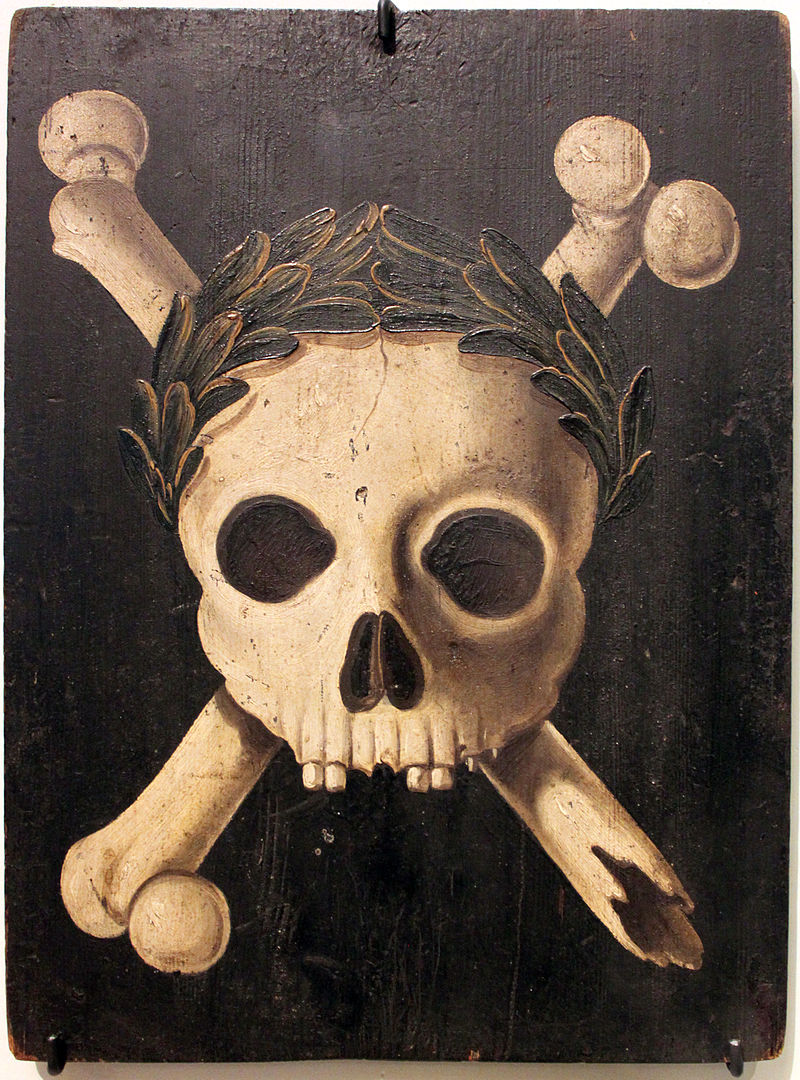
\includegraphics[width = 100mm, height = 80mm]{images/german-plague-panel.jpg}
			\caption{Plague Panel: The Triumph of Death. (1635). Germany.}
		\end{figure}
	\end{frame}

    \begin{frame}{Some Heuristics Metrics on Pandemics}
    	\begin{itemize}
    		\item \textbf{$R_0$ Value}: An average number of cases, an infected person will cause in their infection period.\\
    			\begin{align*}
		    		&R^{Measles}_{0} \in [12,18] \quad&\cite{R0-measles}\\
		    		&R^{SARS. CoV. 2}_{0} \approx 5.7\quad&\cite{R0-COV19}\\
		    		&R^{SARS}_{0} \in  [0.19,1.08]\quad&\cite{R0-SARS}\\
		    		&R^{Common Cold}_{0} \in [2,3]\quad&\cite{R0-CommonCold}\\
		    		&R^{MERS}_{0} \in [0.3, 0.8]\quad&\cite{R0-MERS}
    			\end{align*}
    	\end{itemize}  
    \end{frame}
	
    \begin{frame}
    	
		    	
    \end{frame}

    \begin{frame}{References}
        \footnotesize{
        \begin{thebibliography}{}
       		\bibitem[Guerra et al.]{R0-measles} Guerra, F. M., Bolotin, S., Lim, G., Heffernan, J., Deeks, S. L., Li, Y., \& Crowcroft, N. S. (2017). The basic reproduction number (R0) of measles: a systematic review. The Lancet Infectious Diseases, 17(12), e420-e428.
       		
       		\bibitem[Sanche et al.]{R0-COV19} Sanche, S., Lin, Y. T., Xu, C., Romero-Severson, E., Hengartner, N., \& Ke, R. (2020). Early Release-High Contagiousness and Rapid Spread of Severe Acute Respiratory Syndrome Coronavirus 2.
       		
       		\bibitem[Freeman et al.]{R0-CommonCold} Freeman, Colin. (2020). Magic formula that will determine whether Ebola is beaten. The Telegraph. Telegraph.Co.Uk. 
       		
       		\bibitem[Kucharski et al.]{R0-MERS} Kucharski, A. J., \& Althaus, C. (2015). The role of superspreading in Middle East respiratory syndrome coronavirus (MERS-CoV) transmission. Euro surveillance, 20(25), pii-21167.
       		
       		\bibitem[Chowell et al.]{R0-SARS} Chowell, G., Castillo-Chavez, C., Fenimore, P. W., Kribs-Zaleta, C. M., Arriola, L., \& Hyman, J. M. (2004). Model parameters and outbreak control for SARS. Emerging Infectious Diseases, 10(7), 1258.
        \end{thebibliography}
    }
    \end{frame}
    
\end{document}
